\section{ARCHITECTURAL DESIGN}

\subsection{Overview: High level components and their interaction}
\noindent\makebox[\textwidth][c]{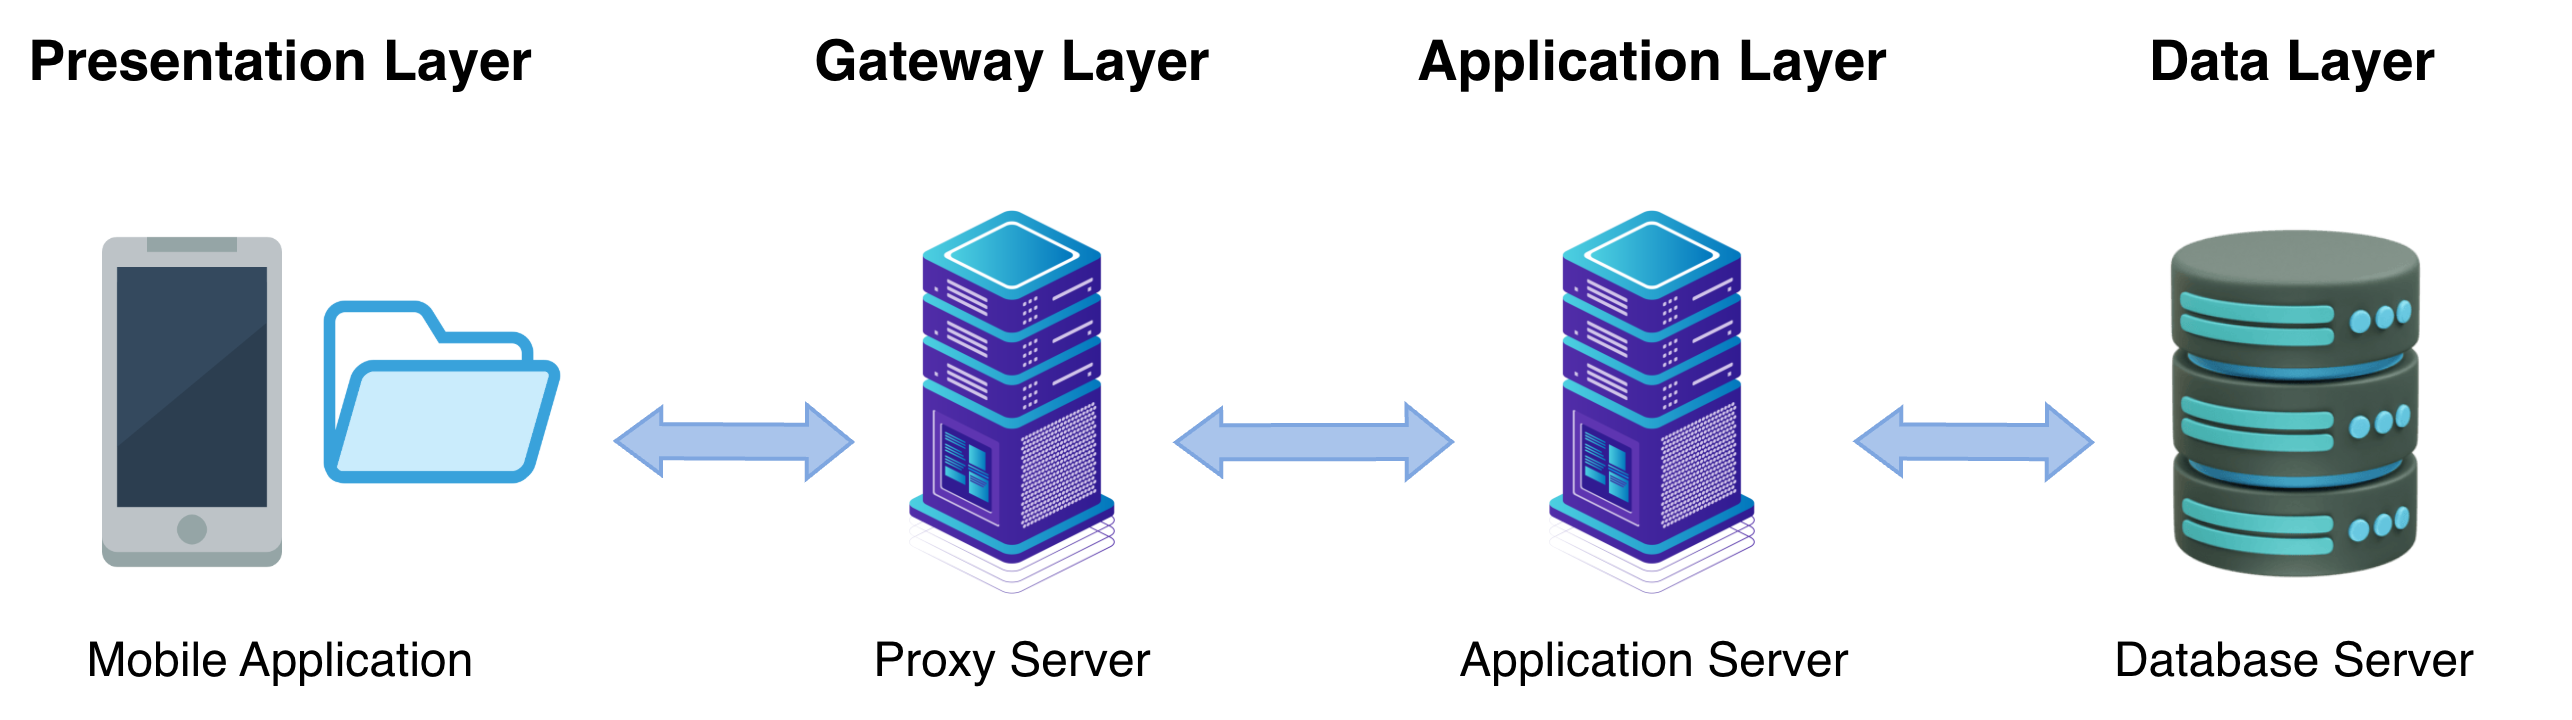
\includegraphics[width=1.1\textwidth]{images/InformalDiagram.png}}
\subsection{Component view}
%Introduzione generale ai componenti. Architettura client-server 3 livelli (min) distribuita
%Server distribuiti geograficamente. GUI e salvataggi percorsi privati esclusivamente in locale (dunque parte del db in locale)
%Ricerca dei percorsi tramite server

\begin{itemize}
    \item \textbf{User Management Service}
    \item \textbf{Automated Path Data Collection Service}
    \item \textbf{Path Data Transformation Service} %trasforma i dati raw collezionati dai sensori in un formato human readable
    \item \textbf{Meteorological Data Retrieval Service}
    \item \textbf{Path Research Service} %unico riservato anche a utenti non registrati
    \item \textbf{Path Publication Service}
    \item \textbf{Manual Path Insertion Service}
    \item \textbf{Inventory Handling Service}
\end{itemize}

\newpage
\subsection{Deployment view}
This chapter describes the deployment view of the BPP system. it outlines the execution
environment of the system and details the gegraphical distribution of the hardware components that host the
software making up the application. 
\noindent\makebox[\textwidth][c]{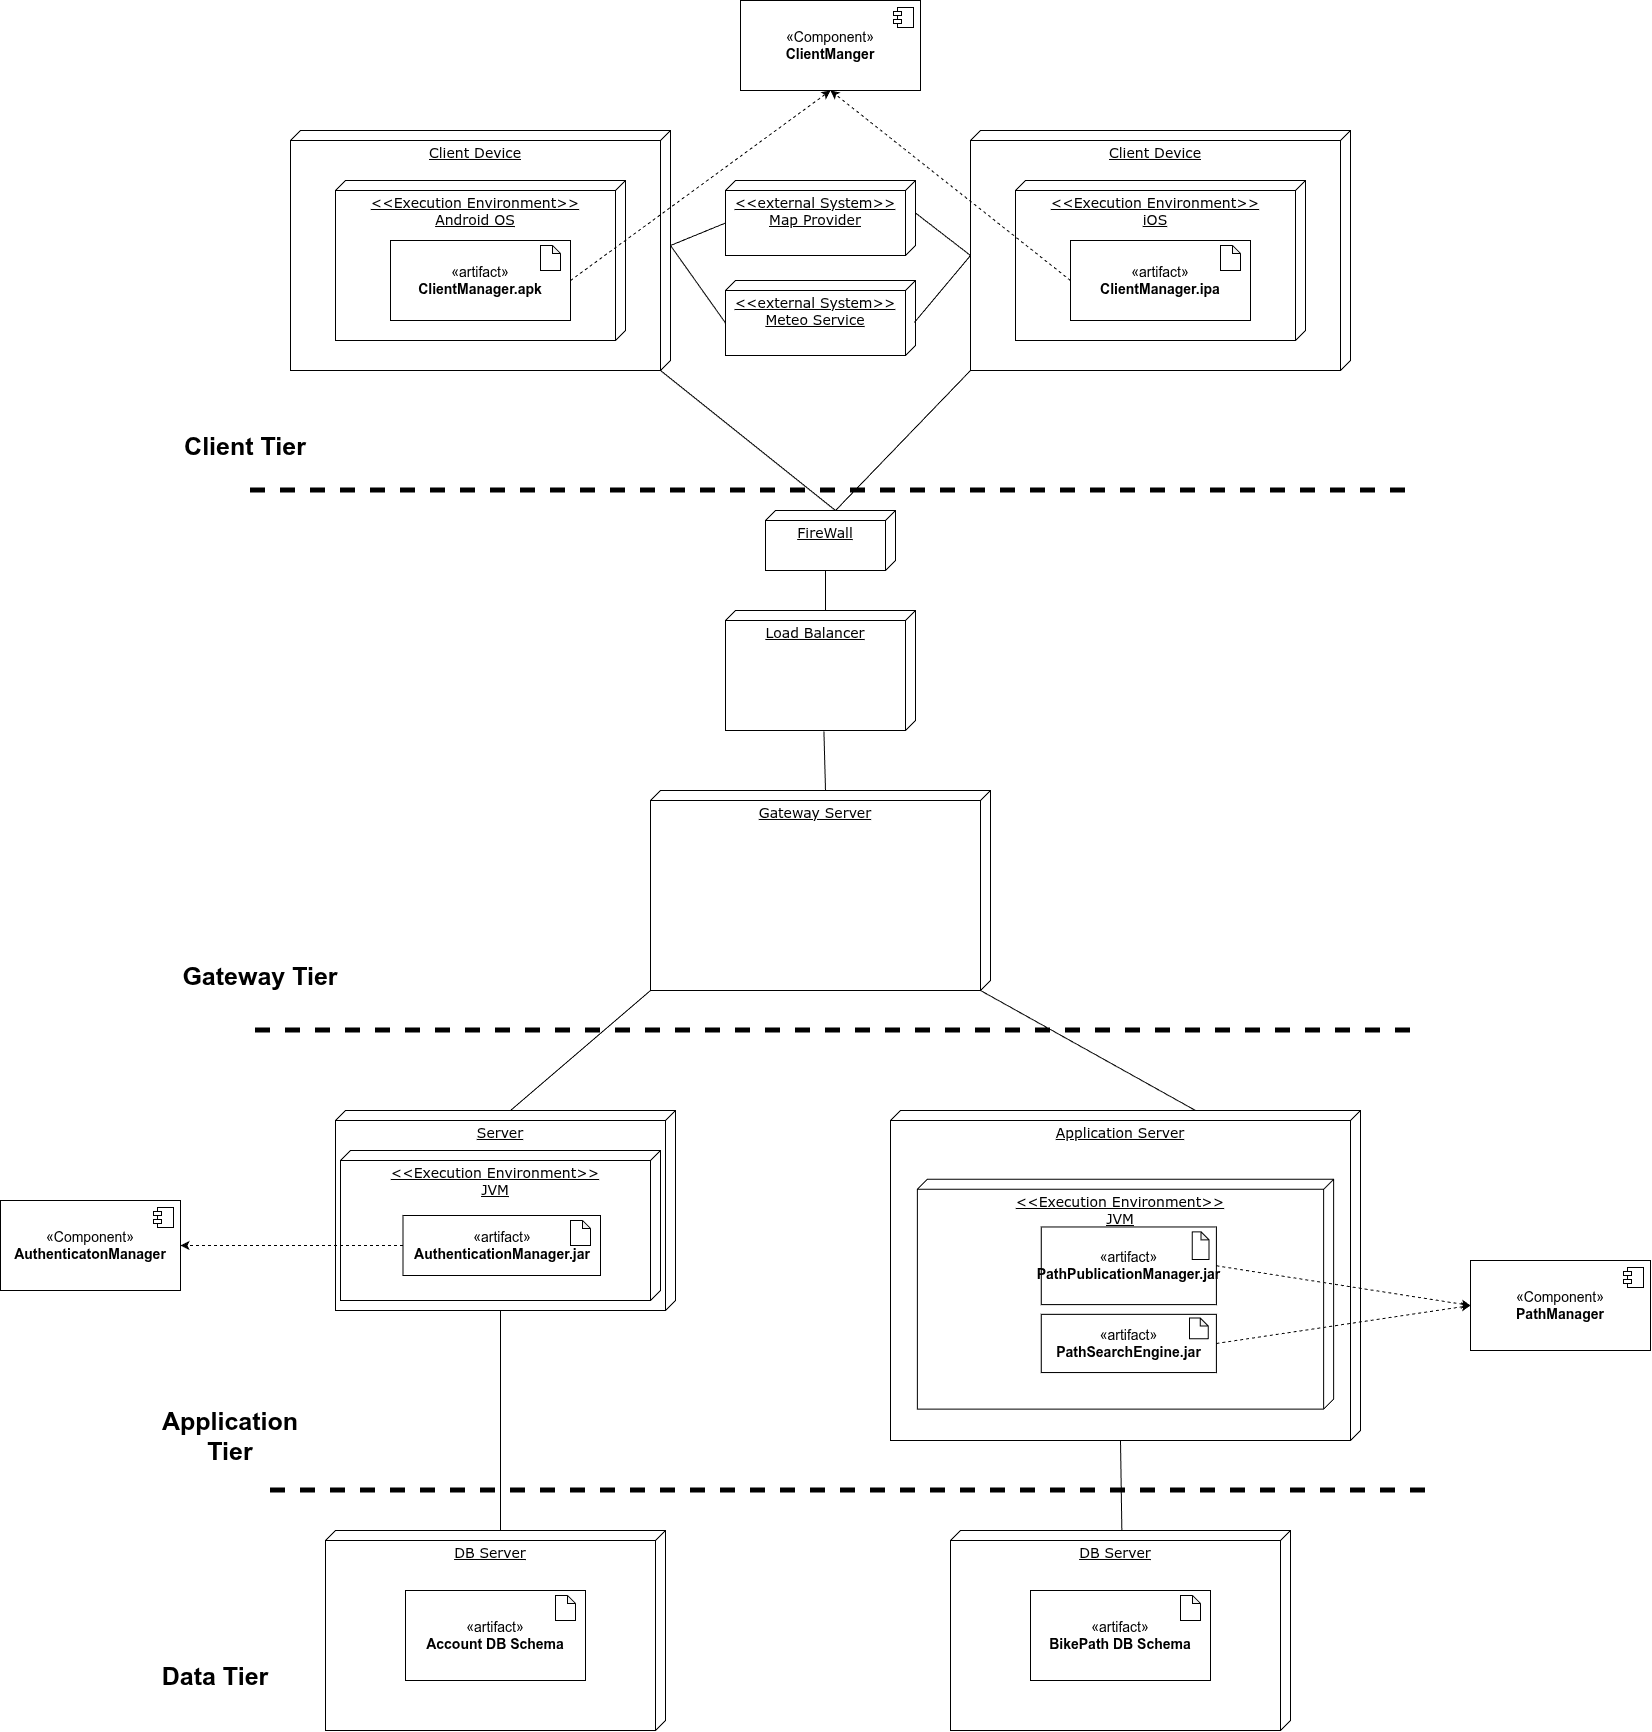
\includegraphics[width=1.1\textwidth]{images/Deployment_Diagram.drawio.png}}

\newpage \noindent The deployment architecture follows a Four-Tier approach. The first tier is a Thick Client able to provide parts of the functionalities (gathering of
information and offline storage) also when it is not connected to the Server. \newline\newline
The second tier consists of the Gateway and the Load balancer. The Gateway exposes the public endpoint and route the requests toward the 
correct type of service (Account Server or Application Server). This layer works also as shield against external treats. The communication between first and second tier takes
place via HTTPS protocol.\newline\newline
The third tier consist of two types of servers: The ones to manage all the things regarding the personal account of a user and the ones that regard the "shared" part of the application, i.e. the publication of bike paths.
This separation between the two aspect allow to easily achieve independent scalability of the two type of service, and allow the system to avoid the congestion of both service if only one is managing a big quantity of requests. In other words this kind of
separation introduces a high level of decoupling.
The fourth and last tier is dedicated to the Data, the databases do not communicate directly with internet but only with the Servers responsible to manage the information.\newline
The communication between these tiers takes place via TCP/IP protocol.\newline\newline

We proceed to provide further details about the elements in the graph. \newline\newline



\begin{itemize}
    \item \textbf{Database Server for Published Paths} \\
    This database stores all the published paths by registered users.
    The system shall be highly available and shall be able to provide eventual consistency across all the
    replicas, so all the set of available paths will be visible to all the users around the world.
    \item \textbf{Database Server for Registered Users} \\
    This Database stores all the personal information of registered users such as name, e-mail and the hashed password.
    \item \textbf{Application Server}\\
    This Server is responsible to process all the requests regarding the publication and the search of bike path from the final user.
    This component manipulates data, and then it has direct access to the related Database.
    \item \textbf{Account Server}\\
    This Server is responsible to manage all the request that regard the accounts of the end user and the related information.
    This component manipulates personal data of the users, and then it has access to the related Database.
    \item \textbf{Load Balancer} \\
    It distributes incoming requests across multiple Gateway to optimize system performances and avoid to overloading one server.
    \item \textbf{Firewall}\\ %Ops... non ci sono nel deployment diagram <-- Sistema
    Monitors incoming network traffic, blocking potentially harmful packets before they reach the system. Positioned before the load balancers it creates
    a safe perimeter around the network.
    \item \textbf{Mobile Device} \\
    This represents the device used by the end user. It requires the app installed in order to access the BPP application. 
\end{itemize}
\subsection{Runtime view}
\subsection{Component interfaces}
\subsection{Selected architectural styles and patterns}
\subsection{Other design decisions}